% Created 2020-12-08 二 23:15
% Intended LaTeX compiler: xelatex
\documentclass[11pt]{report}
\usepackage{graphicx}
\usepackage{grffile}
\usepackage{longtable}
\usepackage{wrapfig}
\usepackage{rotating}
\usepackage[normalem]{ulem}
\usepackage{amsmath}
\usepackage{textcomp}
\usepackage{amssymb}
\usepackage{capt-of}
\usepackage{hyperref}
\author{曹嘉祺 PB18030874 化学与材料科学学院 有机化学系 \thanks{中国 安徽合肥 中国科学技术大学 Email: \href{mailto:mkq@mail.ustc.edu.cn}{mkq@mail.ustc.edu.cn}}}
\usepackage[scheme=plain]{ctex}
\usepackage{fontspec}
\setmainfont{更纱黑体 UI SC}
\hypersetup{colorlinks=true,linkcolor=blue}
\usepackage{longtable}
\date{\today}
\title{燃烧热的测定}
\hypersetup{
 pdfauthor={曹嘉祺 PB18030874 化学与材料科学学院 有机化学系},
 pdftitle={燃烧热的测定},
 pdfkeywords={},
 pdfsubject={},
 pdfcreator={Emacs 27.1 (Org mode 9.4)}, 
 pdflang={English}}
\begin{document}

\maketitle
\tableofcontents

\begin{abstract}
通过苯甲酸为标准,让其在恒温氧弹量热计中完全燃烧,从测得的结果计算(雷诺图
法校正温度)恒温氧弹量热计的热容,然后让萘在相同的恒温氧弹量热计中完全燃烧,
测得萘完全燃烧时的恒容燃烧热,再计算出萘的恒压燃烧热。


\noindent\rule{\textwidth}{0.5pt}
\begin{itemize}
\item 关键词: 燃烧热\quad 氧弹卡计\quad 雷诺校正
\end{itemize}
\end{abstract}
\begin{abstract}
When one mole of certain substance burns completely, the heat it generates
is called enthalpy of combustion. We applied oxygen bull calorimeter after been
measured by benzyl‐acid for measuring Naphthalene’s enthalpy of combustion at
constant volume, and redressed the difference in temperature by Renault figure,
consequently calculated its enthalpy of combustion at constant pressure.

\noindent\rule{\textwidth}{0.5pt}

\begin{itemize}
\item key words:  heat capacity, oxygen bomb calorimeter, Renault picture
\end{itemize}
\end{abstract}
\part{前言}
\label{sec:org1c433be}
\chapter{实验原理}
\label{sec:org72bebbf}
\section{燃烧热的测定原理}
\label{sec:org8f459db}
燃烧热的定义是:一摩尔的物质完全燃烧时所放出的热量。
所谓完全燃烧,即组成反应物的各元素,在经过燃烧反应后,必须呈显本元素的最高化合价。
如C经燃烧反应后,变成CO,不能认为是完全燃烧。只有在变成CO\textsubscript{2}时,方可认为是完全燃烧。
同时还必须指出,反应物和生成物在指定的温度下都属于标准态。
如苯甲酸在298.15K时的燃烧反应过程为:
\[
    C_{6}H_{5}COOH(s)+\frac{15}{2}O_{2}(g)\longrightarrow 7CO_{2}(g)+3H_{2}O(l)
    \]

由热力学第一定律,恒容过程的热效应Q\textsubscript{V},即\(\Delta\) U。恒压过程的热效应Q\textsubscript{P},即\(\Delta\) H。它们之间的相互关系如下:
\[
    Q_{P}=Q_{V}+\Delta n(RT)
    \]
其中n为反前后气态物质的物质的量之差。R为气体常数。T为反应的绝对温度。

本实验通过测定萘完全燃烧时的恒容燃烧热,然后再计算出萘的恒压燃烧\(\Delta\) H。

在计算萘的恒压燃烧热时,应注意其数值的大小与实验的温度有关,其关系式为:
\[
    \left(\frac{\partial \Delta H}{\partial T}\right)_{p}=\Delta_{r}C_{p}
    \]
式中的\(\Delta\)\textsubscript{r}C\textsubscript{P}是反应前后的恒压热容之差,它是温度的函数。一般说来,
反应的热效应随温度的变化不是很大,在较小的温度范围内,我们可以认为它是一常数。

热是一个很难测定的物理量,热量的传递往往表现为温度的改变。而温度却很容易测量。如果有一种仪器,已知它每升高一度所需的热量,那么,我们就可在这种仪器中进行燃烧反应,
只要观察到所升高的温度就可知燃烧放出的热量。根据这一热量我们便可求出物质的燃烧热。

在实验中我们所用的恒温氧弹量热计(恒温氧弹卡计)就是这样一种仪器。为了测得恒容燃烧热,我们将反应置于一个恒容的氧弹中,为了燃烧完全,在氧弹内充入20个左右大气压的纯氧。这一装置的构造将在下面做详细介绍。

为了确定量热卡计每升高一度所需要的热量,也就是量热计的热容,可用通电加热法或标准物质法。
本实验用标准物质法来测量量热卡计的热容即确定仪器的水当量。这里所说的标准物质为苯甲酸,
其恒容燃烧时放出的热量为26460 J\(\cdot\) g\textsuperscript{-1}。实验中将苯甲酸压片准确称量并扣除Cu-Ni合金丝的质量后与该数值的乘积即为所用苯甲酸完全燃烧放出的热量。
Cu-Ni合金丝燃烧时放出的热量及实验所用O\textsubscript{2}气中带有的N\textsubscript{2}气燃烧生成氮氧化物溶于水,
所放出的热量的总和一并传给卡计使其温度升高。
根据能量守恒原理,物质燃烧放出的热量全部被氧弹及周围的介质(本实验为3000毫升水)等所吸收,
得到温度的变化为\(\Delta\) T,所以氧弹卡计的热容为:
\[
    C_{卡}=\frac{Q}{\Delta T}=\frac{mQ_{v}+2.9l+5.98V}{\Delta T}
    \]
式中:
\begin{itemize}
\item m为苯甲酸的质量(准确到110-5克)
\item l为燃烧掉的Cu-Ni合金丝的长度(cm)
\item 2.9为每厘米Cu-Ni合金丝燃烧放出的热量单位(J\(\cdot\) cm\textsuperscript{-1})
\item V为滴定燃烧后氧弹内的洗涤液所用的0.1mol\(\cdot\) dm\textsuperscript{-3}的NaOH溶液的体积(本次不需要)
\item 5.98为消耗1mL 0.1 mol\(\cdot\) dm\textsuperscript{-3}的NaOH所相当的热量(单位为J)。由于此项结果对QV的影响甚微,所以常省去不做。
\end{itemize}

确定了仪器(含3000mL水)热容,我们便可根据公式求出欲测物质的恒容燃烧热Q\textsubscript{V},即:
\[
    Q_{V}=(C_{卡}\Delta T-2.9l)/m\times M
    \]
然后求得该物质的恒压燃烧热Q\textsubscript{P},即\(\Delta\) H。

\section{用雷诺作图法校正\(\Delta\) T}
\label{sec:org0f435e4}

尽管在仪器上进行了各种改进,但在实验过程中仍不可避免环境与体系间的热量传递。这种传递使得我们不能准确地由温差测定仪上读出由于燃烧反应所引起的温升\(\Delta\) T。而用雷诺作图法进行温度校正,能较好地解决这一问题。

将燃烧前后所观察到的水温对时间作图,可联成FHIDG折线,如下图所示。图4-1中H相当于开始燃烧之点。
D为观察到的最高温度。在温度为室温处作平行于时间轴的JI线。它交折线FHIDG于I点。
过I点作垂直于时间轴的ab线。然后将FH线外延交ab线于A点。将GD线外延,交ab线于C点。
则AC两点间的距离即为\(\Delta\) T。图中AA′为开始燃烧到温度升至室温这一段时间\(\Delta\) t\textsubscript{1}内,
由环境辐射进来以及搅拌所引进的能量而造成量热计的温度升高。
它应予以扣除之。CC′为温度由室温升高到最高点D这一段时间\(\Delta\) t\textsubscript{2}内,
量热计向环境辐射而造成本身温度的降低。它应予以补偿之。因此AC可较客观的反应出由
于燃烧反应所引起量热计的温升。在某些情况下,量热计的绝热性能良好,热漏很小,
而搅拌器的功率较大,不断引进能量使得曲线不出现极高温度点,如图4-2,校正方法相似。

\begin{center}
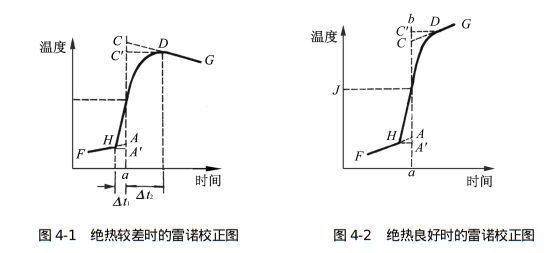
\includegraphics[width=.9\linewidth]{../img/1.png}
\end{center}

必须注意,应用这种作图法进行校正时,卡计的温度与外界环境的温度不宜相差太大(最好不超过2-3\textsuperscript{o}C),否则会引入大的误差。

\part{实验部分}
\label{sec:org321dc3e}
\chapter{实验仪器与试剂}
\label{sec:orgb174def}
\section{仪器}
\label{sec:org4e2faf4}
\begin{center}
\begin{tabular}{lll}
仪器 & 数目 & 厂家/备注\\
\hline
GR3500型氧弹式量热计 & 1套 & 长沙仪器厂\\
JDW-3F精密电子温差测定仪 & 1台 & \\
南京大学应用物理研究所 &  & \\
燃烧热数据采集接口装置BH-2S 型 & 1台 & 南大万和\\
压片机 & 1台 & \\
万用表 & 1个 & \\
扳手 & 1把 & \\
氧气钢瓶 &  & 需大于80kg压力\\
铁丝 & 若干 & \\
容量瓶 & 2个 & \\
\end{tabular}
\end{center}


\section{试剂}
\label{sec:org538d842}
\begin{center}
\begin{tabular}{ll}
试剂 & 厂家\\
\hline
苯甲酸(分析纯) & 国药集团化学试剂有限公司\\
萘(分析纯) & 国药集团化学试剂有限公司\\
 & \\
\end{tabular}
\end{center}
\chapter{仪器介绍}
\label{sec:org0cf643a}
\begin{center}
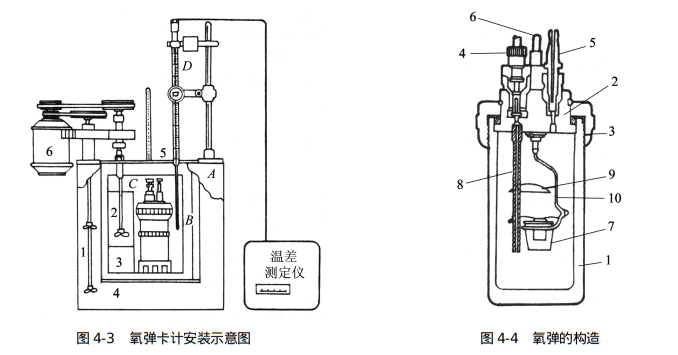
\includegraphics[width=.9\linewidth]{../img/2.png}
\end{center}
图4-3中,内筒C以内的部分为仪器的主体,即为本实验研究的体系,体系C与外界以空气层B绝热,
下方有绝缘的垫片4架起,上方有绝热胶板5敷盖。为了减少对流和蒸发,减少热辐射及控制环境温度恒定,
体系外围包有温度与体系相近的水套A。为了使体系温度很快达到均匀,还装有搅拌器2,由马达6带动。
为了准确测量温度的变化,我们由精密的温差测定仪来实现。实验中把温差测定仪的热敏探头插入研究体系内,
便可直接准确读出反应过程中每一时刻体系温度的相对值。
样品燃烧的点火由一拨动开关接入一可调变压器来实现,设定电压在24V进行点火燃烧。

图4-4是氧弹的构造。氧弹是用不锈钢制成的,主要部分有厚壁圆筒1、弹盖2和螺帽3紧密相连;在弹盖2上装有用来充入氧气的进气孔4、排气孔5和电极6,电极直通弹体内部,同时做为燃烧皿7的支架;为了将火焰反射向下而使弹体温度均匀,在另一电极8(同时也是进气管)的上方还有火焰遮板9。

\chapter{实验步骤}
\label{sec:org0fd2294}
\section{量热计水当量的测定}
\label{sec:orgd83a7b9}
\begin{enumerate}
\item 样品压片
\label{sec:org9ac580b}
     压片前先检查压片用钢模是否干净,否则应进行清洗并使其干燥,用台
秤称0.8g 苯甲酸,并用直尺准确量取长度为16cm 左右的细Cu‐Ni 合金丝一根,准确称量并
把其双折后在中间位置打环,置于压片机的底板压模上,装入压片机内,倒入预先粗称的苯
甲酸样品,使样品粉末将合金丝环浸埋,用压片机螺杆徐徐旋紧,稍用力使样品压牢(注意
用力均匀适中,压力太大易使合金丝压断,压力太小样品疏松,不易燃烧完全),抽去模底
的托板后,继续向下压,用干净滤纸接住样品,弹去周围的粉末,将样品置于称量瓶中,在
分析天平上用减量法准确称量后供燃烧使用。 
\item 装置氧弹
\label{sec:org5af48a4}
     拧开氧弹盖,将氧弹内壁擦干净,特别是电极下端的不锈钢接线柱更应
擦干净。在氧弹中加1 毫升蒸馏水。将样品片上的合金丝小心地绑牢于氧弹中两根电极8
与10 上(见图4 氧弹剖面图)。旋紧氧弹盖,用万用电表检查两电极是否通路。若通路,则
旋紧出气口5 后即可充氧气。按图5 所示,连接氧气钢瓶和氧气表,并将氧气表头的导管与氧弹的进气管接通,此时减压阀门2 应逆时针旋松(即关紧),打开氧气钢瓶上端氧气出口阀门1(总阀)观察表一的指示是否符合要求(至少在4MPa),然后缓缓旋紧减压阀门2(即渐渐打开),使表2 指针指在表压2MPa,氧气充入氧弹中。1‐2min 后旋松(即关闭)减压阀门2,关闭阀门1,再松开导气管,氧弹已充入约2MPa 的氧气,可供燃烧之用。但是阀门2 至阀门1 之间尚有余气,因此要旋紧减压阀门2 以放掉余气,再旋松阀门2,使钢瓶和氧气表头复原。

\begin{center}
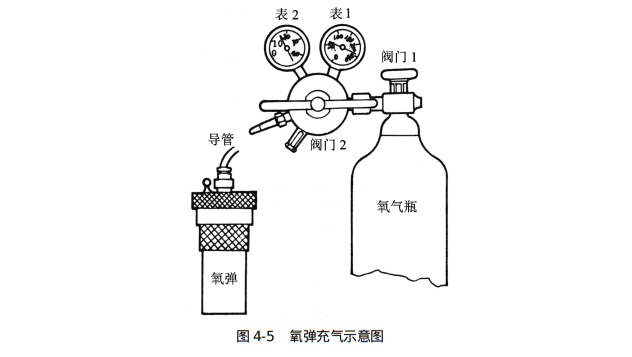
\includegraphics[width=.9\linewidth]{../img/3.png}
\end{center}
\end{enumerate}
\section{燃烧和测量温差}
\label{sec:orgbc365af}
按图将氧弹卡计及内筒,搅拌器装配好。
\begin{enumerate}
\item 用精密电子测量温差仪的热电偶探头准确测量量热计恒温水套A(外套)的实际温度。
\item 打开温差测定仪,让其预热,并将测温探头插入外套测温口中。
\item 在水盆中放入自来水(约4000mL),用热电偶探头测量水盆里的自来水温度,用加冰或加热水的方法调节水温低于外套温度1.4‐1.6\textsuperscript{o}C。
\item 把充好氧气的氧弹放入已事先擦洗干净的内筒C 中。用容量瓶准确量取3000ml 已调好温度的水,置于内筒C 中。
\item 检查点火开关是否置于“关”的位置,插上点火电极,盖上绝热胶木板。
\item 开启搅拌马达,调节温差测定仪设定旋纽,使温差测定仪上指示为1.000,此时对应的实际温度为外套温度。
\item 迅速把测温探头置于内筒C 上端的测温口中,观察温差测定仪的读数,一般10min后应在‐0.85 左右,然后点火。(太低或太高都要重新调节水温,以保证外套水温在燃烧升温曲线的中间位置)。报时器每半分钟响一次,响时即记录温差测定仪上温度的读数,至少读20‐30min。
\item 插好点火电源,将点火开关置于“开”的位置并立即拨回“关”的位置。在几十秒内温差测定仪的读数骤然升高,继续读取读数,直至读数平稳(约25 个数,每半分钟一次。如果在1‐2 分钟内,温差测定仪的读数没有太大的变化,表示样品没有燃烧,这时应仔细检查,请教老师后再进行处理)。停止记录,拔掉点火电源。
\item 取出氧弹,打开放气阀,排出废气,旋开氧弹盖,观察燃烧是否完全,如有黑色残渣,则证明燃烧不完全,实验需重新进行。如燃烧完全,量取剩余的铁丝长度,根据公式计算C\textsubscript{卡}的值。如需精确测量,还需在装置氧弹时加1mL蒸馏水于氧弹内,燃烧后将弹体用蒸馏水清洗,用0.1 mol\(\cdot\) dm\textsuperscript{‐3}NaOH 滴定之。
\end{enumerate}
\section{萘恒容燃烧热的测定}
\label{sec:org1c34abb}
称取0.6 克的萘,按上述操作步骤,压片、称重、燃烧等实验操作重复一次。测量萘的
恒容燃烧热Q\textsubscript{V},并根据公式计算Q\textsubscript{P},即为\(\Delta\) H,并与手册作比较,计算实验的相对误差。
\chapter{实验数据及数据处理(见附件)}
\label{sec:org71493dd}
\chapter{结果分析与讨论}
\label{sec:org6d45bf5}
\section{实验结果}
\label{sec:org76fc4f1}
计算得到体系的热容为:
\[
    C_{卡}=14403.93J/K
    \]
萘的恒容燃烧热为:
\[
    Q_{Vm萘}=
    \frac{C_{卡}\Delta T-2.9l}{m}\times M=
    5.1755\times 10^{6}J/mol
    \]
萘的恒压燃烧热为:
\[
    Q_{P}=Q_{V}+\Delta n(RT)=5.1755\times 10^{6}+2\times 8.314 \times (273.15+10.549)=
    5.1802\times 10^{6}J/mol
    \]
相对误差:
\[
    D=\frac{5.1802-5.1388}{5.1388}\times 100\%=0.81\%
    \]
\section{实验讨论}
\label{sec:org761bb19}
\begin{enumerate}
\item 误差分析
\label{sec:orge896f6c}
通过附件中对燃烧热误差传导的分析,发现其实度误差影响最大的是雷诺校正图上温度
的取点,而其他的条件,诸如质量、温度计读数误差,都相对比较小。下面列出实验中的一
些问题,及影响:
\begin{enumerate}
\item 通过用 gnuplot 拟合一组数据,与 Origin 拟合的结果相比较,虽然外推线的方程不完全一样 (主要是斜率的有效数字取位问题) ,但是以此计算出的外推点差的也很少,由于 gnuplot拟合有便利脚本操作优点,所以我选用的是gnuplot拟合;这对于实验结果的影响与Origin 差得很少。
\item 在压片之后成质量,由于要在氧弹中系好已称好的样品,这个过程中可能会有损失,造成最终计算结果偏小;所以,在压好之后要擦去样品表面的碎末。
\item 控制恒温槽温度是实验的难点,在实验前后,温度分别低于、高于外界温度,且差的不太多,利于温度补偿,这个很难准确做到。
\item 尽管在实验时在不断地搅拌水,但水温达到完全均匀几乎不可能,在记录数据时,很明显的可以看到示数的跳动,这可能是造成误差的一个原因。
\end{enumerate}
\item 实验总结
\label{sec:org3141cf6}

\begin{enumerate}
\item 为了确保点火的成功,一方面,要及时用万用表检查氧弹里点火线情况,另一方面,要在点火的细节上做好功夫,诸如,点火线的形状,在文献\textsubscript{[3]}中提到了一种点火线的设计,如图:
\begin{center}
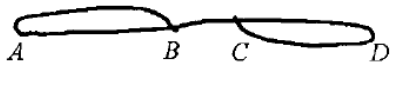
\includegraphics[width=.9\linewidth]{../img/4.png}
\end{center}中间部分弯成螺旋形,这很类似于在实验中实际采用的点火线形状,设计成有沟槽的形状便于固定在氧弹内部。
\item 有些文献对于实验室采用萘作为测定物质提出质疑,因为据称萘有轻微的致癌性,对于这样的化学物质可以做一些改进,其中,改用蔗糖,测其燃烧的热就是一个方案;具体的测量数据也说明这样的方案可以很好地作为替代品,测得比较准确的数据。
\end{enumerate}
\end{enumerate}

\part{参考文献}
\label{sec:orgc6f1e7d}
\begin{enumerate}
\item 崔献英,柯燕雄,单绍纯.物理化学实验[M].合肥:中国科学技术大学出版社,2000.4
\item 傅献彩,沈文霞,姚天扬.物理化学.第四版.北京:高等教育出版社,1990.10
\item 燃烧热测定实验研究 李森兰 杜巧云等 大学化学 第 16 卷 第 1 期 2001 年2 月
\item 李震. 氧弹式量热法测燃烧热实验的改进.大学化学,2001.8
\item 维基百科数据库.
\item 燃烧热测定实验中三条直线校正温度法的研究 王岩 袁悦等 实验室科学 第 14 卷第 1 期 2011 年 2 月
\item 对燃烧热的测定的改进 天津科技大学理学院吴法伦 赵妍等 中国轻工教育2006 专刊
\end{enumerate}
\part{附录: 数据处理过程}
\label{sec:org58417cf}
\chapter{原始数据}
\label{sec:orgde4f96c}
\section{其他数据}
\label{sec:orgbd01ac0}
点火用Cu‐Ni 合金丝的线密度 0.9983 mg\(\cdot\) cm\textsuperscript{‐1}
\begin{enumerate}
\item 苯甲酸
\label{sec:org75d240b}
\begin{itemize}
\item m丝=0.0224g
\item m总=0.8089g
\item T粗=10.338°C
\item T初=10.355°C
\item T末=10.488°C
\item m丝剩=0.0175g
\item 烧掉的金属丝=0.0224g-0.0175g=0.0049g
\item 苯甲酸重=0.8089g-0.0224g=0.7865g
\end{itemize}
\item 萘
\label{sec:orge6ec0bd}
\begin{itemize}
\item m丝=0.0221g
\item m总=0.6151g
\item T粗=10.532°C
\item T初=10.515°C
\item T末=10.583°C
\item m丝剩=0.0178g
\item 烧掉的金属丝=0.0221g-0.0178g=0.0043g
\item 萘重=0.6151g-0.0221g=0.5930g
\end{itemize}
\end{enumerate}
\section{温度曲线}
\label{sec:orgbfc646f}
\begin{enumerate}
\item 苯甲酸
\label{sec:org16b1aba}
\begin{center}
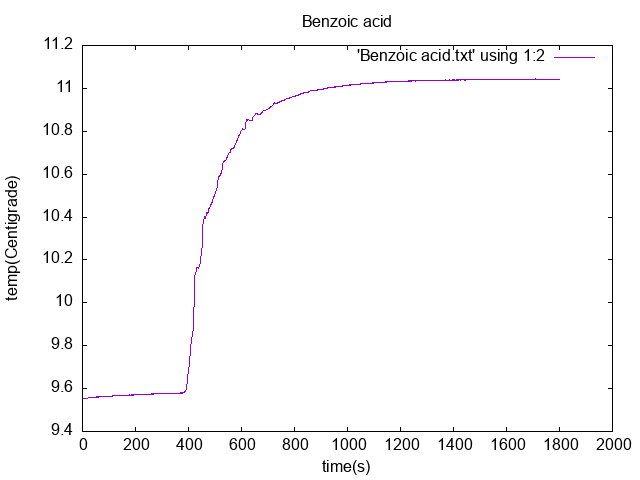
\includegraphics[width=.9\linewidth]{../img/苯甲酸.png}
\end{center}
\item 萘
\label{sec:orged11961}
\begin{center}
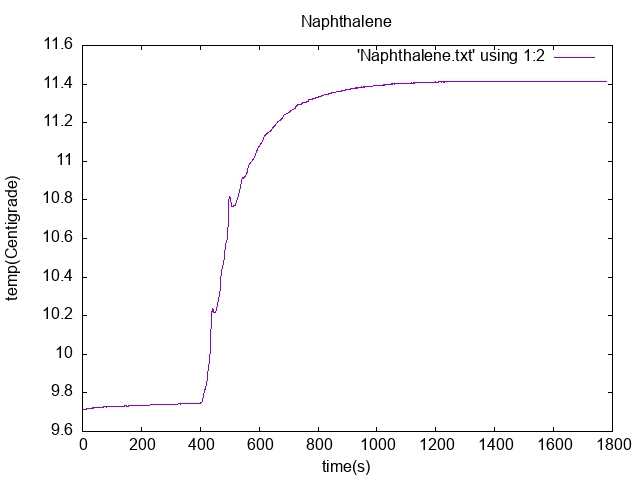
\includegraphics[width=.9\linewidth]{../img/萘.png}
\end{center}
\end{enumerate}
\chapter{数据处理}
\label{sec:orge117420}
\section{仪器热容的测定(14403.93J/K)}
\label{sec:org96388b1}
\begin{enumerate}
\item 外桶平均温度的计算(10.422\textsuperscript{o}C)
\label{sec:orgd5211e6}
\[
     t=\frac{T_{初}+T_{末}}{2}=10.422^{o}C
     \]
\item 找到图中对应时间(475s)
\label{sec:orgff745d9}
下表节选自原始数据
\begin{center}
\begin{tabular}{rr}
时间(s) & 温度(\textsuperscript{o}C)\\
\hline
471 & 10.420\\
472 & 10.419\\
473 & 10.418\\
474 & 10.419\\
475 & 10.423\\
476 & 10.429\\
477 & 10.440\\
478 & 10.442\\
\end{tabular}
\end{center}
可见最接近10.422\textsuperscript{o}C的时间为475s
\item 对直线部分进行线性拟合
\label{sec:orgaafce6c}
分别取前300组数据点和后300组数据点进行直线拟合:
\begin{center}
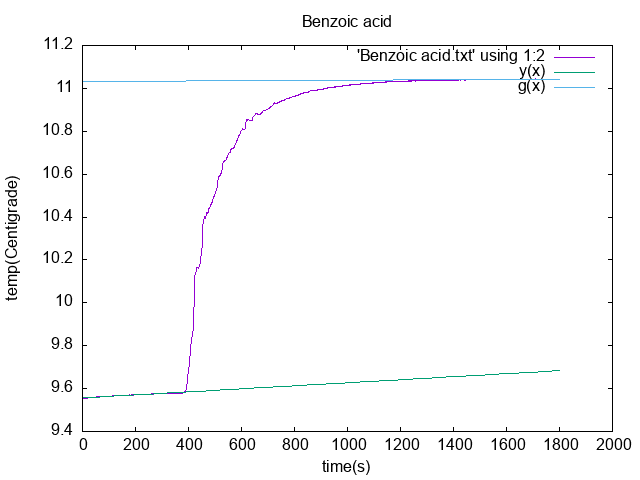
\includegraphics[width=.9\linewidth]{../img/Benzoic acid.png}
\end{center}

拟合结果如下:
\begin{enumerate}
\item 前300个点(9.5901\textsuperscript{o}C)
\label{sec:org0fabb50}
\begin{verbatim}
gnuplot> fit y(x) '苯甲酸前300.txt' via k,b
iter      chisq       delta/lim  lambda   k             b            
   0 8.1236473947e+06   0.00e+00  1.23e+02    9.984963e-01  -6.975280e-01
   1 7.8348539973e+03  -1.04e+08  1.23e+01    5.272032e-02  -6.751147e-01
   2 5.0680384376e+03  -5.46e+04  1.23e+00    4.120690e-02   1.315657e+00
   3 8.0081100113e+00  -6.32e+07  1.23e-01    1.705808e-03   9.229005e+00
   4 2.6621267809e-04  -3.01e+09  1.23e-02    7.131695e-05   9.556446e+00
   5 2.6484159617e-04  -5.18e+02  1.23e-03    7.064034e-05   9.556582e+00
   6 2.6484159617e-04  -5.47e-09  1.23e-04    7.064034e-05   9.556582e+00
iter      chisq       delta/lim  lambda   k             b            

After 6 iterations the fit converged.
final sum of squares of residuals : 0.000264842
rel. change during last iteration : -5.46519e-14

degrees of freedom    (FIT_NDF)                        : 298
rms of residuals      (FIT_STDFIT) = sqrt(WSSR/ndf)    : 0.000942725
variance of residuals (reduced chisquare) = WSSR/ndf   : 8.8873e-07

Final set of parameters            Asymptotic Standard Error
=======================            ==========================
k               = 7.06403e-05      +/- 6.285e-07    (0.8897%)
b               = 9.55658          +/- 0.0001091    (0.001142%)

correlation matrix of the fit parameters:
#                k      b      
k               1.000 
b              -0.867  1.000 

\end{verbatim}
\[
Temp=7.06403\times 10^{-5}t+9.55658
\]
t=475s时:
\[
Temp=9.5901^{o}C
\]
\item 后300个点(11.0349\textsuperscript{o}C)
\label{sec:orge1569ac}
\begin{verbatim}
gnuplot> fit g(x) '苯甲酸后300.txt' via l,c
iter      chisq       delta/lim  lambda   l             c            
   0 8.1500817116e+08   0.00e+00  1.17e+03    1.000000e+00   1.000000e+00
   1 2.3112173854e+03  -3.53e+10  1.17e+02    7.710539e-03   9.994066e-01
   2 8.4561020403e+01  -2.63e+06  1.17e+01    6.067330e-03   1.000023e+00
   3 8.3530184714e+01  -1.23e+03  1.17e+00    6.030245e-03   1.061358e+00
   4 3.2019704721e+01  -1.61e+05  1.17e-01    3.735850e-03   4.858821e+00
   5 8.2739900256e-03  -3.87e+08  1.17e-02    6.571061e-05   1.093329e+01
   6 8.0951999789e-05  -1.01e+07  1.17e-03    6.057991e-06   1.103202e+01
   7 8.0951783348e-05  -2.67e-01  1.17e-04    6.048294e-06   1.103203e+01
iter      chisq       delta/lim  lambda   l             c            

After 7 iterations the fit converged.
final sum of squares of residuals : 8.09518e-05
rel. change during last iteration : -2.6737e-06

degrees of freedom    (FIT_NDF)                        : 300
rms of residuals      (FIT_STDFIT) = sqrt(WSSR/ndf)    : 0.000519461
variance of residuals (reduced chisquare) = WSSR/ndf   : 2.69839e-07

Final set of parameters            Asymptotic Standard Error
=======================            ==========================
l               = 6.04829e-06      +/- 3.429e-07    (5.669%)
c               = 11.032           +/- 0.0005667    (0.005137%)

correlation matrix of the fit parameters:
#                l      c      
l               1.000 
c              -0.999  1.000 

\end{verbatim}
\[
Temp=6.04829\times 10^{-6}t+11.032
\]
t=475时
\[
Temp=11.0349^{o}C
\]
\end{enumerate}
\item 计算\(\Delta\) T(1.4448\textsuperscript{o}C)
\label{sec:org25ea4da}
\[
     \Delta T=11.0349^{o}C-9.5901^{o}C=1.4448^{o}C
     \]
\item 计算体系热容(14403.93J/K)
\label{sec:org86c0cf3}
\[
     C_{卡}=
     \frac{Q}{\Delta T}=
     \frac{mQ_{V}+2.9l+5.98V}{\Delta T}=
     \frac{0.7865\times 26460+2.9\times(0.0049/0.9983)}{1.4448}=
     14403.93J/K
     \]
\end{enumerate}

\section{萘燃烧热的测定(5.1802\texttimes{} 10\textsuperscript{6}J/mol)}
\label{sec:orge155317}
\begin{enumerate}
\item 外桶平均温度的计算(10.549\textsuperscript{o}C)
\label{sec:org2899003}
\[
     t=\frac{T_{初}+T_{末}}{2}=10.549^{o}C
     \]
\item 找到图中对应时间(484s)
\label{sec:org15d4db5}
下表节选自原始数据
\begin{center}
\begin{tabular}{rr}
时间(s) & 温度(\textsuperscript{o}C)\\
\hline
483 & 10.535\\
484 & 10.546\\
485 & 10.559\\
\end{tabular}
\end{center}

可见最接近10.549\textsuperscript{o}C的时间为484s

\item 对直线部分进行线性拟合
\label{sec:orgc274064}
分别取前300组数据点和后300组数据点进行直线拟合:
\begin{center}
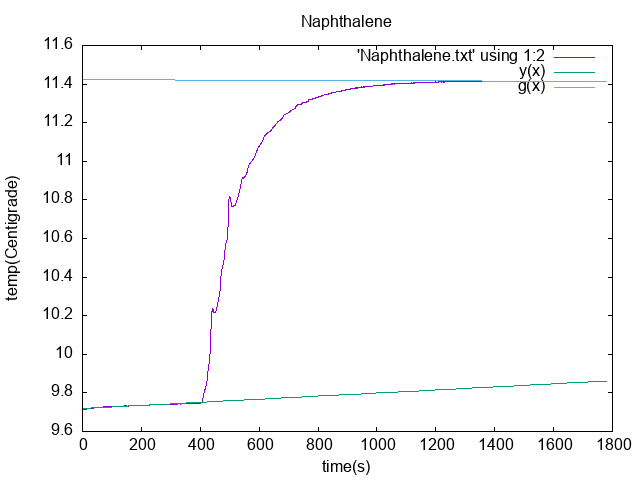
\includegraphics[width=.9\linewidth]{../img/Naphthalene.png}
\end{center}
拟合结果如下:
\begin{enumerate}
\item 前300个点(9.7579\textsuperscript{o}C)
\label{sec:org47499fb}
\begin{verbatim}
gnuplot> fit y(x) '萘前300.txt' via k,b      
iter      chisq       delta/lim  lambda   k             b            
   0 8.0767310735e+00   0.00e+00  6.76e+00    7.064034e-05   9.556582e+00
   1 1.0638114985e-03  -7.59e+08  6.76e-01    7.064395e-05   9.720378e+00
   2 1.0323975239e-03  -3.04e+03  6.76e-02    7.086504e-05   9.720618e+00
   3 8.6567862077e-04  -1.93e+04  6.76e-03    7.725728e-05   9.719656e+00
   4 8.5047097691e-04  -1.79e+03  6.76e-04    7.984658e-05   9.719266e+00
   5 8.5047072738e-04  -2.93e-02  6.76e-05    7.985711e-05   9.719265e+00
iter      chisq       delta/lim  lambda   k             b            

After 5 iterations the fit converged.
final sum of squares of residuals : 0.000850471
rel. change during last iteration : -2.93407e-07

degrees of freedom    (FIT_NDF)                        : 298
rms of residuals      (FIT_STDFIT) = sqrt(WSSR/ndf)    : 0.00168936
variance of residuals (reduced chisquare) = WSSR/ndf   : 2.85393e-06

Final set of parameters            Asymptotic Standard Error
=======================            ==========================
k               = 7.98571e-05      +/- 1.126e-06    (1.41%)
b               = 9.71926          +/- 0.0001956    (0.002012%)

correlation matrix of the fit parameters:
#                k      b      
k               1.000 
b              -0.867  1.000 

\end{verbatim}
\[
Temp=7.98571\times 10^{-5}t+9.71926
\]
t=484s时:
\[
Temp=9.7579^{o}C
\]


\item 后300个点(11.4204\textsuperscript{o}C)
\label{sec:orgffce876}
\begin{verbatim}
gnuplot> fit g(x) '萘后300.txt' via l,c
iter      chisq       delta/lim  lambda   l             c            
   0 3.9160389603e+01   0.00e+00  7.80e+00    6.048294e-06   1.103203e+01
   1 4.1016011044e-04  -9.55e+09  7.80e-01    6.048465e-06   1.140402e+01
   2 2.8743621315e-04  -4.27e+04  7.80e-02    6.047221e-06   1.140468e+01
   3 2.8237391827e-04  -1.79e+03  7.80e-03    5.924213e-06   1.140488e+01
   4 1.0801597275e-04  -1.61e+05  7.80e-04    1.312973e-07   1.141439e+01
   5 5.8330176499e-05  -8.52e+04  7.80e-05   -4.979681e-06   1.142277e+01
   6 5.8326308558e-05  -6.63e+00  7.80e-06   -5.025171e-06   1.142285e+01
   7 5.8326308558e-05  -7.95e-08  7.80e-07   -5.025175e-06   1.142285e+01
iter      chisq       delta/lim  lambda   l             c            

After 7 iterations the fit converged.
final sum of squares of residuals : 5.83263e-05
rel. change during last iteration : -7.95242e-13

degrees of freedom    (FIT_NDF)                        : 280
rms of residuals      (FIT_STDFIT) = sqrt(WSSR/ndf)    : 0.000456408
variance of residuals (reduced chisquare) = WSSR/ndf   : 2.08308e-07

Final set of parameters            Asymptotic Standard Error
=======================            ==========================
l               = -5.02518e-06     +/- 3.339e-07    (6.644%)
c               = 11.4228          +/- 0.0005484    (0.004801%)

correlation matrix of the fit parameters:
#                l      c      
l               1.000 
c              -0.999  1.000 
\end{verbatim}
\[
Temp=-5.02518\times 10^{-6}t+11.4228
\]
t=484s时:
\[
Temp=11.4204^{o}C
\]
\end{enumerate}
\item 计算\(\Delta\) T(1.6625\textsuperscript{o}C)
\label{sec:orgb783127}
\[
     \Delta T=11.4204^{o}C-9.7579^{o}C=1.6625^{o}C
     \]

\item 计算萘的恒压燃烧热(5.1802\texttimes{} 10\textsuperscript{6}J/mol)
\label{sec:orgb887f1d}
\[
     C_{卡}=
     \frac{Q}{\Delta T}=
     \frac{mQ_{V}+2.9l+5.98V}{\Delta T}=
     \frac{0.5930\times Q_{V萘}+2.9\times(0.0043/0.9983)}{1.6625}=
     14403.93J/K
     \]
\[
     Q_{Vm萘}=
     \frac{C_{卡}\Delta T-2.9l}{m}\times M=
     5.1755\times 10^{6}J/mol
     \]
\[
     Q_{P}=Q_{V}+\Delta n(RT)=5.1755\times 10^{6}+2\times 8.314 \times (273.15+10.549)=
     5.1802\times 10^{6}J/mol
     \]
\item 误差计算(0.81\%)
\label{sec:org7226bae}
查阅资料知萘的标准恒压燃烧热:
\[
     Q_{Pm萘}= 5.1388\times 10^6 J/mol
     \]

相对误差:
\[
     D=\frac{5.1802-5.1388}{5.1388}\times 100\%=0.81\%
     \]
\end{enumerate}
\end{document}
